\documentclass[authoryear, twocolumn]{elsarticle}
\usepackage{lmodern}
\usepackage{amssymb,amsmath}
\usepackage{ifxetex,ifluatex}
\usepackage{fixltx2e} % provides \textsubscript
\ifnum 0\ifxetex 1\fi\ifluatex 1\fi=0 % if pdftex
  \usepackage[T1]{fontenc}
  \usepackage[utf8]{inputenc}
\else % if luatex or xelatex
  \ifxetex
    \usepackage{mathspec}
  \else
    \usepackage{fontspec}
  \fi
  \defaultfontfeatures{Ligatures=TeX}
\fi
% use upquote if available, for straight quotes in verbatim environments
\IfFileExists{upquote.sty}{\usepackage{upquote}}{}
% use microtype if available
\IfFileExists{microtype.sty}{%
\usepackage{microtype}
\UseMicrotypeSet[protrusion]{basicmath} % disable protrusion for tt fonts
}{}
\usepackage[unicode=true]{hyperref}
\hypersetup{
            pdftitle={The link between tongue root advancement and the voicing effect: an ultrasound study of Italian and Polish},
            pdfborder={0 0 0},
            breaklinks=true}
%\urlstyle{same}  % don't use monospace font for urls
\usepackage{natbib}
\bibliographystyle{plainnat}
\IfFileExists{parskip.sty}{%
\usepackage{parskip}
}{% else
\setlength{\parindent}{0pt}
\setlength{\parskip}{6pt plus 2pt minus 1pt}
}
\setlength{\emergencystretch}{3em}  % prevent overfull lines
\providecommand{\tightlist}{%
  \setlength{\itemsep}{0pt}\setlength{\parskip}{0pt}}
\setcounter{secnumdepth}{5}
% Redefines (sub)paragraphs to behave more like sections
\ifx\paragraph\undefined\else
\let\oldparagraph\paragraph
\renewcommand{\paragraph}[1]{\oldparagraph{#1}\mbox{}}
\fi
\ifx\subparagraph\undefined\else
\let\oldsubparagraph\subparagraph
\renewcommand{\subparagraph}[1]{\oldsubparagraph{#1}\mbox{}}
\fi

% set default figure placement to htbp
%\makeatletter
%\def\fps@figure{htbp}
%\makeatother

\frenchspacing
\usepackage{cleveref}
\setcitestyle{aysep={},notesep={:},citesep={,}}
\usepackage{ctable}
\author[mcr]{Stefano Coretta\corref{cor1}}
\cortext[cor1]{Corresponding author \ead{stefano.coretta@manchester.ac.uk}}
\address[mcr]{University of Manchester, Linguistics and English Language}

\title{The link between tongue root advancement and the voicing effect: an
ultrasound study of Italian and Polish}
\date{}

\begin{document}
\maketitle

\section{Introduction}\label{introduction}

\label{s:intro}

This paper reports on a previously undocumented link between tongue root
advancement in the production of voiced stops and longer duration of the
preceding vowels. Using ultrasonic data from speakers of Italian and
Polish, I demonstrate that the presence of tongue root advancement
correlates with that of the so-called voicing effect, whereby vowels
tend to be longer before voiced than before voiceless stops. I further
suggest that such correlation points to a new articulatory account of
vowel duration as a covariate of consonantal voicing, by which tongue
root advancement is proposed as a plausible diachronic precursor of the
voicing effect.

A extensive number of studies show that vowels tend to be longer when
followed by voiced obstruents than when they are followed by voiceless
obstruents
\citep{house1953, chen1970, klatt1973, lisker1974, farnetani1986, fowler1992, hussein1994, esposito2002, lampp2004, durvasula2012}.
This phenomenon, know as the voicing effect, has been reported in a
variety of languages, including (but not limited to) English, German,
Hindi, Russian, Italian, Arabic, and Korean (see \citealt{maddieson1976}
for a more comprehensive list). A common stance in the literature is
that the magnitude of the voicing effect differs depending on the
language (although see \citealt{laeufer1992}), and that this phenomenon
is not a universal tendency, since the duration of vowels is not
affected by the voicing of the following obstruents in some languages,
like Polish and Czech \citep{keating1984}. Although several attempts
have been made to explain the voicing effect, an account that survives
all empirical data is still lacking \citep{durvasula2012}.

To provide a rationale for the language-specificity of the voicing
effect, \citet{kluender1988} propose that the source of the effect rests
on the level of the perceptual system. They argue that speakers actively
manipulate vowel durations to enhance the closure-duration difference
which can cue the voicing distinction in obstruents. However,
\citet{fowler1992} shows by means of perceptual experiments that
speakers judge vowels to be longer if the consonant closure duration is
increased, and that, vice versa, consonant closure is perceived to be
longer when vowel duration is increased. Fowler thus refutes on
empirical grounds that speakers exploit durational contrasts to enhance
voicing distinctions. Crucially, \citet{davis1989} demonstrate that
closure duration is not employed as a cue to voicing, fact that further
confutes accounts based on closure-duration enhancement.

A desirable account of the voicing effect should then satisfy both of
the following requirements: (1) it should allow for a language-specific
implementation of the voicing effect, and (2) it should place the source
of the effect in articulatory properties of voiced or voiceless
obstruents that could favour longer or shorter vowel durations. One of
the first articulatory accounts to be proposed points to differences in
the adjustment of the glottis before voiced and voiceless stops
(\citealt{halle1967}, reiterated in \citealt{chomsky1968}).
\citet{halle1967} state that the glottal configuration during voicing in
vowels is different from that of the closure of voiced consonants. Their
argument is that vowels are longer before voiced consonants so that more
time is available to the glottis to achieve a position suitable for
maintaining within-closure voicing. This guarantees that such
configuration is secured before the onset of the consonant closure.
Later studies, however, established that the glottal configuration of
voicing in obstruents does not differ from the one in vowels
\citep{lisker1974,kagaya1975}. Hence, the claim that vowels are longer
to allow glottal adjustments cannot be supported empirically.

A known articulatory difference between voiced and voiceless consonants
regards instead a supra-glottal rather than a laryngeal gesture, namely
the position of the tongue root along the front-back plane of the oral
tract. It has been observed that the tongue root is in a more advanced
position in voiced than in voiceless stops
\citep{kent1969,perkell1969,westbury1983}. This gesture has been
interpreted as a mechanism to ensure voicing during closure. The
realisation of vocal fold vibration (i.e.~voicing) requires the air
pressure in the supra-glottal cavity to be lower than the air pressure
below the glottis. During the production of voiced obstruents, the
supra-glottal pressure quickly increases. Such pressure increase can
hinder the ability to maintain voicing during closure, to the point that
voicing can cease if the supra-glottal pressure is higher than the
sub-glottal pressure \citep{ohala2011}. An articulatory solution to
counterbalance the increase in pressure is to expand the supra-glottal
cavity by advancing the root of the tongue.

Drawing on ultrasound tongue imaging data, \citet{ahn2016} show that
tongue root advancement not only favours voicing in English voiced
steps, but it also facilitates a short lag VOT in the tense stops of
Korean. The established link between voicing, VOT duration, and tongue
root advancement on one hand, and between voicing and vowel duration on
the other, raises the question of whether a correlation exists between
tongue root advancement and vowel duration. If tongue root advancement
plays a role in determining the presence or development of the voicing
effect, then it is expected that voiced consonants should be articulated
with tongue root advancement in voicing-effect languages, but not in
languages without the voicing effect.

For this study ultrasonic tongue data were recorded from speakers of
Italian and Polish, two languages that have been reported to have and
lack the voicing effect respectively. In an investigation of the general
properties of segmental durations of Italian, \citet{farnetani1986} show
that the first vowel in /lada/ is on average 35 milliseconds longer than
the vowel in /lata/ (\(\bar{x}\) = 223 ms, sd = 18 in /lata/;
\(\bar{x}\) = 258 ms, sd = 13 in /lada/, \citealt[26]{farnetani1986}).
\citet{esposito2002} extends Farnetanis's research to all the vowels and
stops of Italian and confirms that vowels are longer when followed by a
voiced stop, with an estimated mean duration similar to that reported in
\citet{farnetani1986}. As for Polish, although a difference of 2
milliseconds in vowel duration can be observed (167.5 ms in /rata/,
169.5 ms in /rada/), such difference has been deemed as non-significant
according to statistical testing \citep{keating1984}. Vowels in Polish
are thus not affected by the voicing of the following consonant.

Based on the hypothesis that tongue root advancement correlates with the
voicing effect (and hence with vowel duration), the expectations with
regard to Italian and Polish are the following: (1) since vowels are
longer before voiced stops in Italian, voiced stops in this language
should be articulated with tongue root advancement, and (2) given that
vowels before voiceless and voiced stops in Polish are about the same
duration, the position of the tongue root in voiced stops should not
differ from that of voiceless stops.

\section{Methodology}\label{methodology}

\subsection{Participants}\label{participants}

\ctable[caption = Sociolinguistic information on participants. The right-most column indicates whether the participant spent more than 6 consecutive months abroad.,
label = t:participants
]{lllll}{}{
\FL
\textbf{id}   & \textbf{sex} & \textbf{age} & \textbf{city}     & \textbf{\textgreater} 6 mo \ML
IT01 & m   & 28  & Verbania & yes               \NN
IT02 & m   & 26  & Udine    & yes               \NN
IT03 & f   & 27  & Verbania & no                \NN
IT04 & f   & 54  & Verbania & no                \NN
PL02 & f   & 32  & Poznań   & yes               \NN
PL03 & m   & 26  & Poznań   & yes               \NN
PL04 & f   & 34  & Warsaw   & no                \NN
PL05 & m   & 34  & Przasnysz & no               \LL
}

Eight native speakers of Italian (2 females, 2 males) and Polish (2
females, 2 males) were recorded in Manchester and in Italy (see
\Cref{t:participants}). The Italian speakers were from Northern Italy
(three from the north-west and one from north-east). The Polish group
was more heterogeneous, with two speakers from the north-west (Poznań),
and two from the north-east (Warsaw and Przasnysz). Ethical clearance
was obtained for this study from the University of Manchester (REF
2016-0099-76). The participants received a small monetary compensation.

\subsection{Equipment set-up}\label{equipment-set-up}

\label{s:equipment}

\begin{figure*}
    \centering
    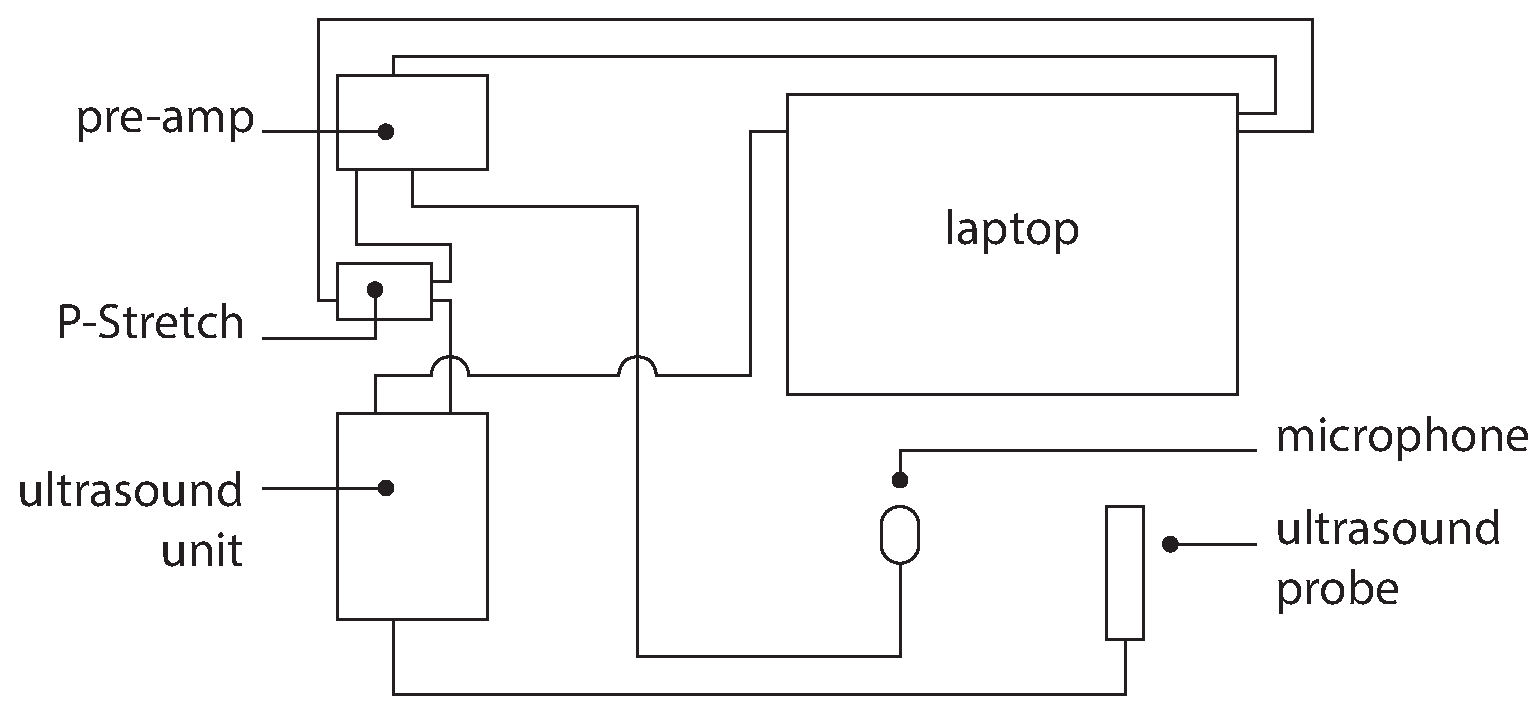
\includegraphics[width=.7\textwidth]{../../graphics/uti-setup.pdf}
    \caption{Schematic representation of the equipment setup (\citealt{articulate2011}). The system is described in details in \Cref{s:equipment}.}
    \label{f:uti-setup}
\end{figure*}

An Articulate Instruments Ltd™ set-up was used for this study
(\Cref{f:uti-setup}). The ultrasonic data was collected through a
TELEMED Echo Blaster 128 unit with a TELEMED C3.5/20/128Z-3 ultrasonic
transducer (20mm radius, 2-4 MHz). A synchronisation unit (P-Stretch)
was plugged into the Echo Blaster unit and used for automatic
audio/ultrasound synchronisation. A FocusRight Scarlett Solo
pre-amplifier and a Movo LV4-O2 Lavalier microphone were used for audio
recording. The acquisition of the ultrasonic and audio signals was
achieved with the software Articulate Assistant Advanced (AAA, v2.17.2)
running on a Hawlett-Packard ProBook 6750b laptop with Microsoft Windows
7. Stabilisation of the ultrasonic transducer was ensured by using a
stabilisation headset produced by Articulate Instruments Ltd™
(\citeyear{articulate2008}).

\subsection{Materials}\label{materials}

Disyllabic words of the form
C\textsubscript{1}V\textsubscript{1}C\textsubscript{2}V\textsubscript{2}
were used as targets, where C\textsubscript{1} = /p/, V\textsubscript{1}
= /a, o, u/, C\textsubscript{2} = /t, d, k, g/, and V\textsubscript{2} =
V\textsubscript{1} (e.g. /pata/, /pada/, /poto/, etc.), giving a total
of 12 target words. A labial stop was chosen as the first consonant to
reduce possible coarticulation with the following vowel (although see
\citealt{vazquez-alvarez2007}). Only coronal and velar stops were used
as target consonants since labial consonants cannot be imaged with
ultrasonography. The target words were embedded in a frame sentence.
Prosodically similar sentences were used to ensure comparability between
languages. The frame sentence was \emph{Dico X lentamente} `I say X
slowly' for Italian, and \emph{Mówię X teraz} `I say X now' for Polish.

\subsection{Procedure}\label{procedure}

The sentences with the target words were randomised for each
participant, although the order was kept the same between repetitions
within participant due to software constraints. Each participant
repeated the list of randomised stimuli six times. A grand total of 576
tokens (288 per language) was recorded. The participant's occlusal plane
was obtained using a bite plate \citep{scobbie2011}, and the hard palate
was imaged by asking the participant to swallow water
\citep{epstein2005}. The frame rate of the acquisition of the ultrasonic
data ranged between 43 and 68 frames per second. Other settings values
varied depending on the frame rate. The ranges of these settings in this
study were: scanlines = 88-114, pixel per scanline = 980-988, field of
view = 71-93, pixel offset = 109-263, depth (mm) = 75-180. The audio
signal was recorded at 22050 MHz (16-bit).

\subsection{Data processing and
analysis}\label{data-processing-and-analysis}

Synchronisation of the ultrasonic and audio signal was achieved in
post-processing, using a built-in procedure of AAA. The audio data were
subject to force alignment using SPPAS \citep{bigi2015}. The outcome of
the automatic annotation was manually corrected after the force
alignment, according to the criteria in \Cref{t:dur-measures}. The onset
of the target consonant burst (C2 burst) was detected automatically in
Praat \citep{boersma2016} by means of the algorithm described in
\citet{ananthapadmanabha2014}. The durations of the following intervals
were extracted from the annotated acoustic landmarks using an automated
procedure in Praat: vowel duration (V1 onset to V1 offset), consonant
duration (V1 offset to V2 onset), and closure duration (V1 offset to C2
burst).

\ctable[caption = List of measurements as extracted from acoustics.,
label = t:dur-measures,
width=\textwidth,
star
]{ll>{\raggedright}p{9cm}}{}{
\FL
\textbf{landmark}               &                  & \textbf{criteria}                                                                                    \ML
vowel onset           & (V1 onset)         & appearance of higher formants in the spectrogram following the burst of /p/ (C1)            \NN
vowel offset          & (V1 offset)        & disappearance of the higher formants in the spectrogram preceding the target consonant (C2) \NN
consonant onset       & (C2 onset)         & corresponds to V1 offset                                                                    \NN
closure onset         & (C2 closure onset) & corresponds to V1 offset                                                                    \NN
consonant offset      & (C2 offset)        & appearance of higher formants of the vowel following C2 (V2); corresponds to V2 onset                                \NN
consonant burst onset & (C2 burst)         & automatic detection \citep{ananthapadmanabha2014}                                           \LL
}

Spline curves were automatically fitted to the visible contours using
the AAA batch tracking function. Manual correction was applied in those
cases that showed clear tracking errors. The time of maximum tongue
displacement within consonant closure was then calculated in AAA
following the method in \citet{strycharczuk2015}. A fan-like frame
consisting of 42 equidistant radial lines was used as the coordinate
system. The origin of the 42 fan-lines coincides with the centre of the
ultrasonic probe, such that each fan-line is parallel to the direction
of the ultrasonic signal. Tongue displacement was thus calculated as the
displacement of the fitted splines along the fan-line vectors. The time
of maximum tongue displacement was the time of greater displacement
along the vector that showed the greatest standard deviation. The vector
search area was restricted to the portion of the splines corresponding
to the tongue tip for coronal consonants, and to the portion
corresponding to the tongue dorsum for velar consonants.

The cartesian coordinates of the tongue contours were exported from two
time points: the onset of C2 closure, and the time of maximum tongue
displacement (which is always within C2 closure). The contours were
normalised within speaker by applying offsetting and rotation relative
to the participant's occlusal plane \citep{scobbie2011}. The durational
data were analysed with linear mixed effects models using \texttt{lme4}
in R \citep{r-core-team2017, bates2015}. P-values were obtained with
likelihood ratio tests comparing the full model with a nested model
without the relevant predictor. Generalised additive mixed models
\citep[GAMMs,][]{wood2006, zuur2012} were used for the statistical
analysis of tongue contour data. Significance testing in GAMMs was
achieved through model comparison with \texttt{itsadug}
\citep{van-rij2017} and visual inspection of the difference smooth, as
suggested in \citet{soskuthy2017}.

\section{Results}\label{results}

The following sections report the results of the durational data
(\Cref{s:vow-duration}), and of the ultrasonic data (\Cref{s:splines})
separately. Given the poor quality of the ultrasonic data for /u/, this
vowel was not included in the statistical analysis of tongue contours,
but the durational data of /u/ were kept in the linear regression
models. The results in \Cref{s:splines} thus refer only to /a/ and /o/.

\subsection{Vowel duration and
voicing}\label{vowel-duration-and-voicing}

\label{s:vow-duration}

A linear mixed effects regression model was fitted to the Italian vowel
duration data with \textsc{vowel duration} (in milliseconds) as the
outcome variable; \textsc{vowel identity} (/a, o, u/), \textsc{voicing}
and \textsc{place of articulation} of the following consonant,
\textsc{sentence duration} (in seconds) as fixed effects;
\textsc{by-speaker} and \textsc{by-word} random \textsc{intercepts}, and
\textsc{by-speaker} random \textsc{coefficients} for voicing. An
interaction between voicing and vowel quality was also included, since
it significantly improved the model. According to the full model as
specified above, Italian vowels are 22 milliseconds longer (se = 6) if
followed by a voiced stop (\(\chi\^2\) = 16.61; p \textless{} 0.001; df
= 3; see \Cref{t:lmer-italian} for a summary of the fixed effects).

For Polish, the same model structure was used, to the exclusion of the
voicing/vowel-identity interaction (which was not significant). Contrary
to previous findings, the model reveals a significant 8 milliseconds
effect (se = 3) of consonantal voicing on the preceding vowel
(\(\chi\^2\) = 5.4; p \textless{} 0.05; df = 1; see \Cref{t:lmer-polish}
for a summary of the fixed effects). Vowel identity and sentence
duration were also significant. The place of C2 significantly improved
the model (\(\chi\^2\) = 6.1; p \textless{} 0.05; df = 1), so it was
included in the full model even though it is deemed as non significant
according to the single predictor p-value (\emph{t} = -2.3; ns; df = 7).
The inspection of the model residuals confirmed the assumptions of
normality and homoscedasticity.

\begin{figure}
    \centering
    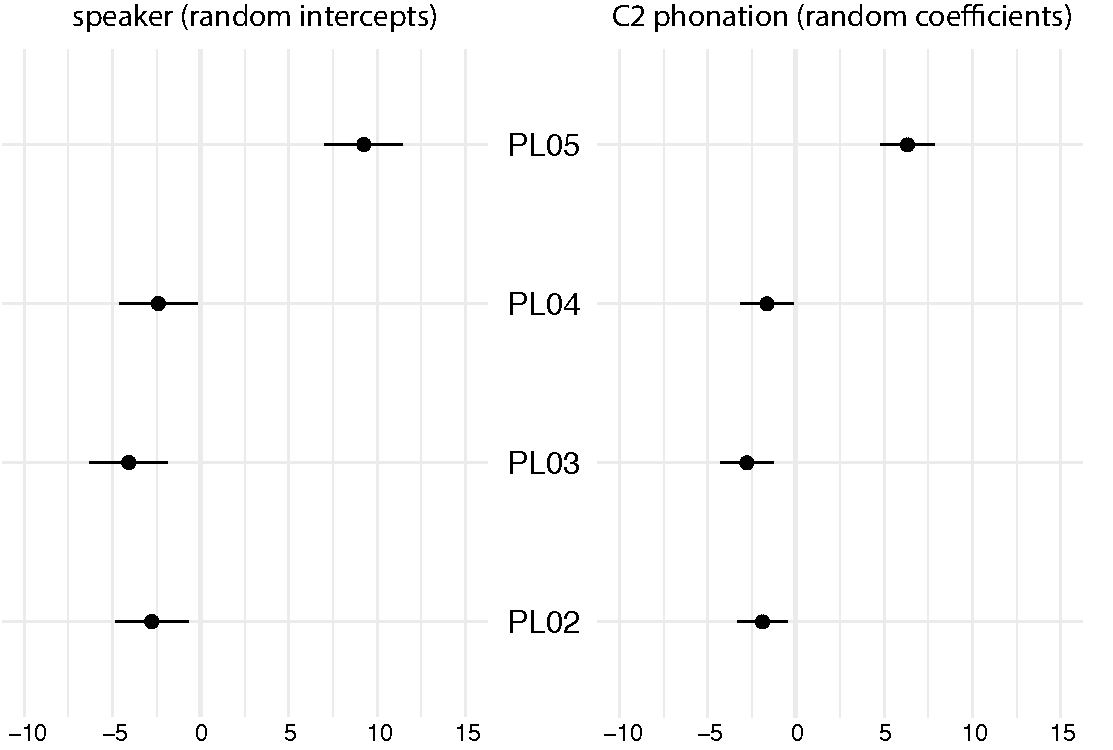
\includegraphics[height=.3\textwidth]{fig/polish-re.pdf}
    \caption{By-speaker random intercepts (left) and coefficients (right) for the effect of C2 voicing on vowel duration in Polish. The higher coefficient estimate (+6.3 ms) for PL05 indicates a relatively stronger effect of voicing for this participant.}
    \label{f:polish-re}
\end{figure}

The exploration of the random coefficients for each speaker indicated
that PL05 has a particularly higher coefficient for voicing, meaning
that the effect of voicing is stronger in his data (\Cref{f:polish-re}).
Note that the exclusion of this speaker from the model doesn't remove
the effect (\(\beta\) = 6 ms; se = 2; \(\chi\^2\) = 8.28; p \textless{}
0.01; df = 1). The estimated effect of voicing on vowel duration for
PL05 was about 14 milliseconds (vowels followed by voiced stops are on
average 14 ms longer in PL05). These observations will become relevant
in the next section, in which the results of the tongue contour data
will be discussed.

\ctable[caption = Summary of fixed effects of the linear mixed-effects regression fitted to the Italian vowel duration data (see \Cref{s:vow-duration} for the model details).,
label = t:lmer-italian
]{lrrrr}{}{
\FL
 & $\beta$ & se  &    df & t \ML
Intercept              &  14.51   &  12.43 & 133.6 &  1.16 \NN
voicing        &  21.84   &   6.07 & 12.7  & 3.59 \NN
place             &  -8.52   &   2.80 & 15.7 & -3.04 \NN
vowel /o/                   &  -8.69   &   4.864 & 15.8 & -1.78 \NN
vowel /u/                   & -29.68   &   4.860 & 15.8 & -6.10 \NN
sent. dur.        &  77.00   &   6.66 & 336.6 & 11.55 \NN
voi:vow /o/ &   2.56   &   6.86 & 15.7 &  0.37 \NN
voi:vow /u/ & -15.57   &   6.86 & 15.7 & -2.26 \LL
}

\ctable[caption = Summary of fixed effects of the linear mixed-effects regression fitted to the Polish vowel duration data (see \Cref{s:vow-duration} for the model details).,
label = t:lmer-polish
]{lrrrr}{}{
\FL
 & $\beta$ & se &      df & t \ML
Intercept       &  22.92   &  10.43 & 127.13  & 2.19 \NN
voicing &   7.88   &   3.25  & 6.860  & 2.41 \NN
vowel (/o/)            & -11.79   &   3.00  & 7.000 & -3.92 \NN
vowel (/u/)            & -29.27   &   3.01  & 7.100 & -9.70 \NN
place      &  -5.57   &   2.45  & 7.00 & -2.27 \NN
sent. dur. &  70.81   &   9.74  & 261.04 &  7.26 \NN
}

\subsection{Tongue contours}\label{tongue-contours}

\label{s:splines}

\begin{figure*}
    \centering
    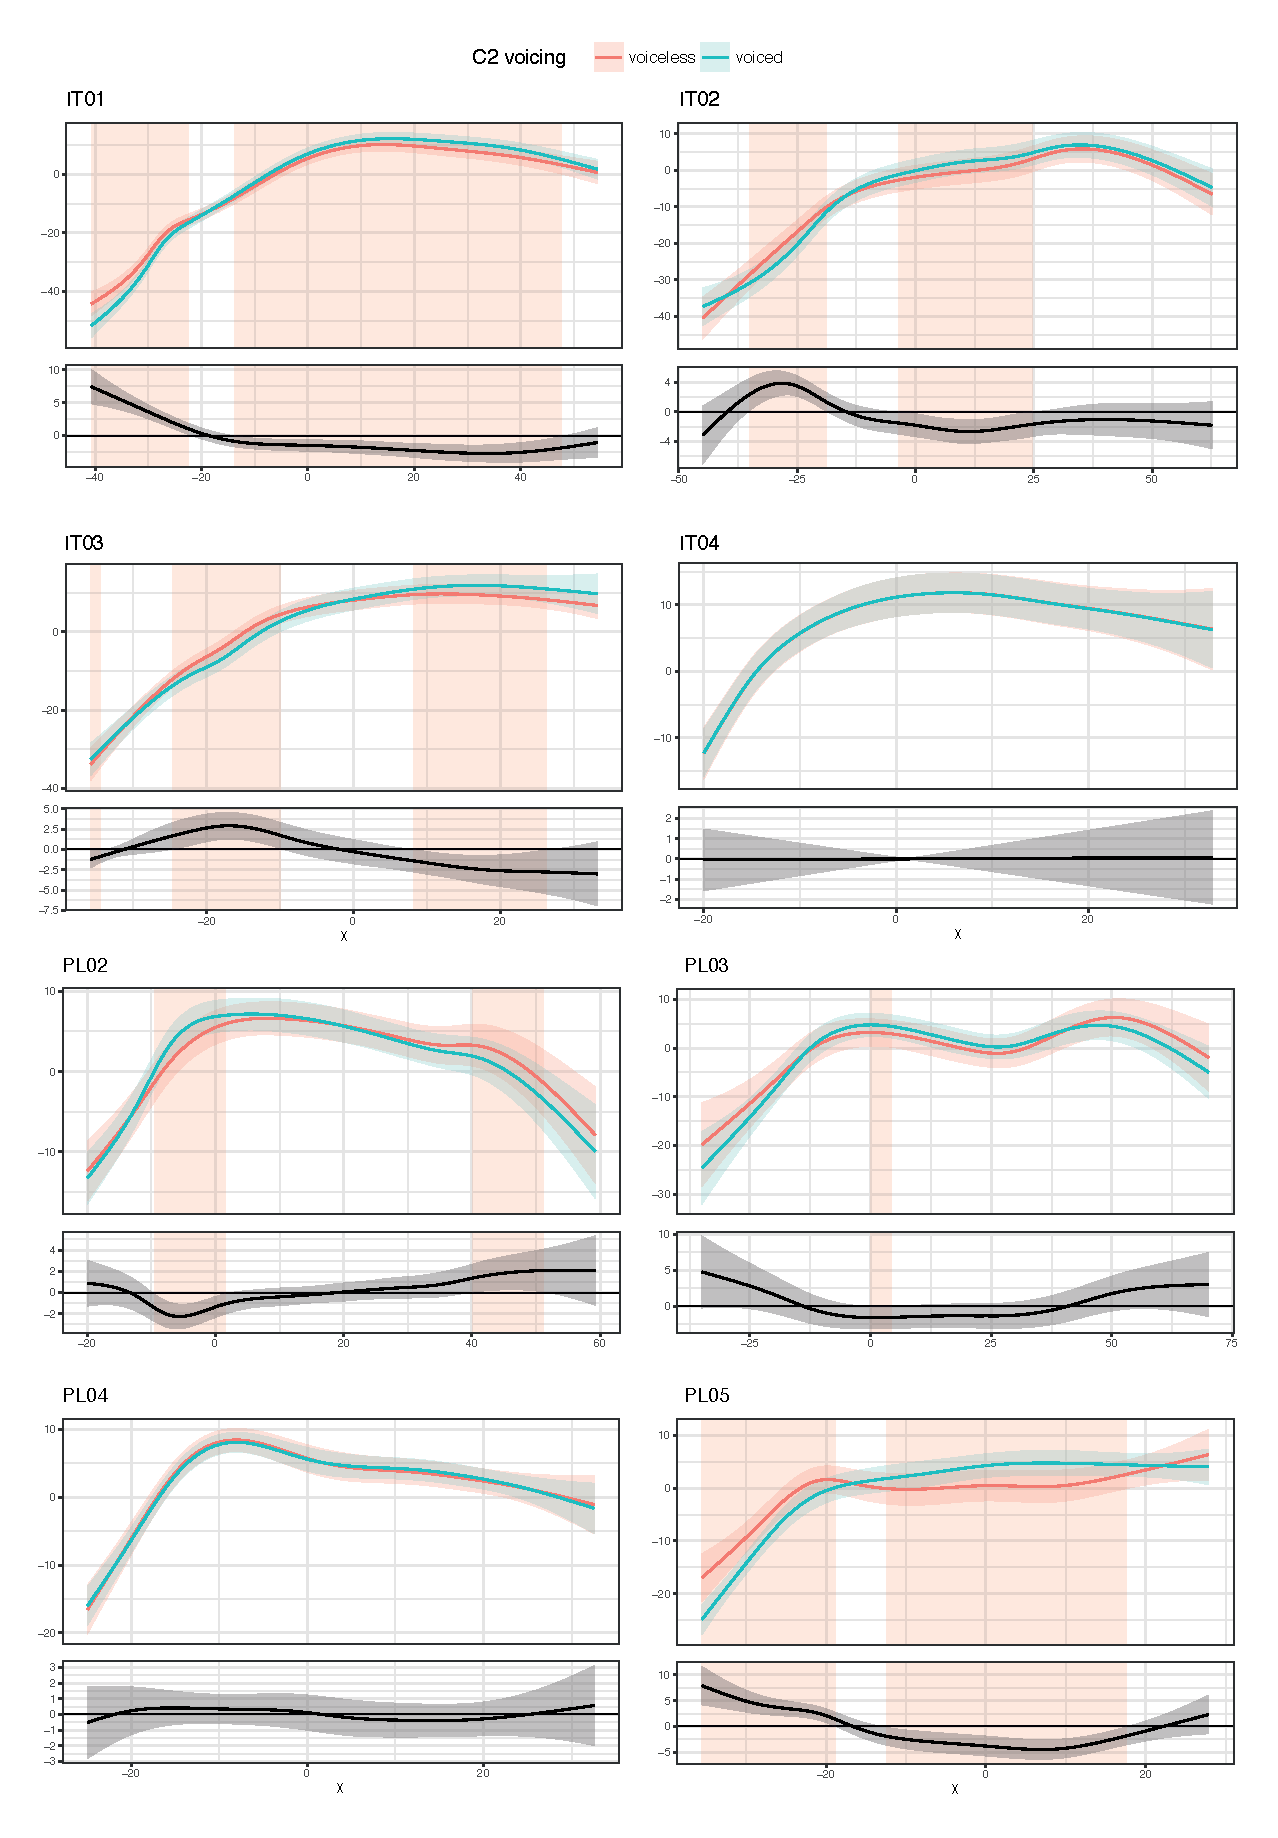
\includegraphics[height=.9\textheight]{fig/tra.pdf}
    \caption{Comparison of tongue contours at the time of maximum tongue displacement (within C2 closure) in Italian (top half) and Polish (bottom half). The plotted contours are the estimated curves in the context of the vowel /a/ followed by coronal consonants. By-voicing difference smooths are shown below the estimated curves. See \Cref{s:splines} for more details.}
    \label{f:tra}
\end{figure*}

GAMMs were fitted to the data of each speaker individually: the
\textsc{y-coordinates} of the contours were included in the model as the
outcome variable; the \textsc{x-coordinates} as the only parametric
term. The following smooths were specified: a reference smooth term for
the x-coordinates, three difference smooths for the x-coordinates by
\textsc{voicing}, \textsc{vowel identity}, and \textsc{place} of
articulation of the following consonant respectively, and
\textsc{by-word} random \textsc{smooths}. A first-order autoregressive
model was included to correct for the high autocorrelation of the
residuals.

The analysis of the Italian ultrasonic data shows that voiced stops are
produced with advancement of the tongue root. \Cref{f:tra} (top half)
shows for each Italian speaker the estimated tongue contours in
voiceless (dashed lines) and voiced stops (continuous lines) at the time
of maximum tongue displacement. Below each tongue contour panel, the
by-voicing difference smooth is also shown (confidence interval in
grey). Tongue contours are significantly different in those points in
which the confidence interval of the difference smooth does not include
0 on the ordinate axis (also indicated by a shaded grey background).

In two participants out of four (IT01, IT02), the root was significantly
more front in voiced stops in both vocalic contexts (/a, o/). On the
other hand, one participant (IT03) had tongue root advancement only in
the context of the vowel /a/, while the fourth participant (IT04) didn't
show advancement at all. For Polish (bottom half of \Cref{f:tra}), three
out of four speakers (PL02, PL03, PL04) did not have tongue root
advancement, while the fourth speaker (PL05) had significant advancement
in voiced stops in both vocalic contexts.

An additional contour analysis was carried out at C2 closure onset for
the Italian and Polish speakers showing advancement. The tongue root at
closure onset was found to be advanced in the voiced consonants of all
these speakers. Comparisons of tongue contours at C2 onset and at the
time of maximum tongue displacement in voiced consonants further
indicated that the degree of root advancement was larger at maximum
displacement for the Italian speakers (IT01, IT02, IT03), but not for
the Polish speaker (PL05). \Cref{f:voiced} exemplifies the results with
the model results from IT01 and PL05.

\begin{figure*}
    \centering
    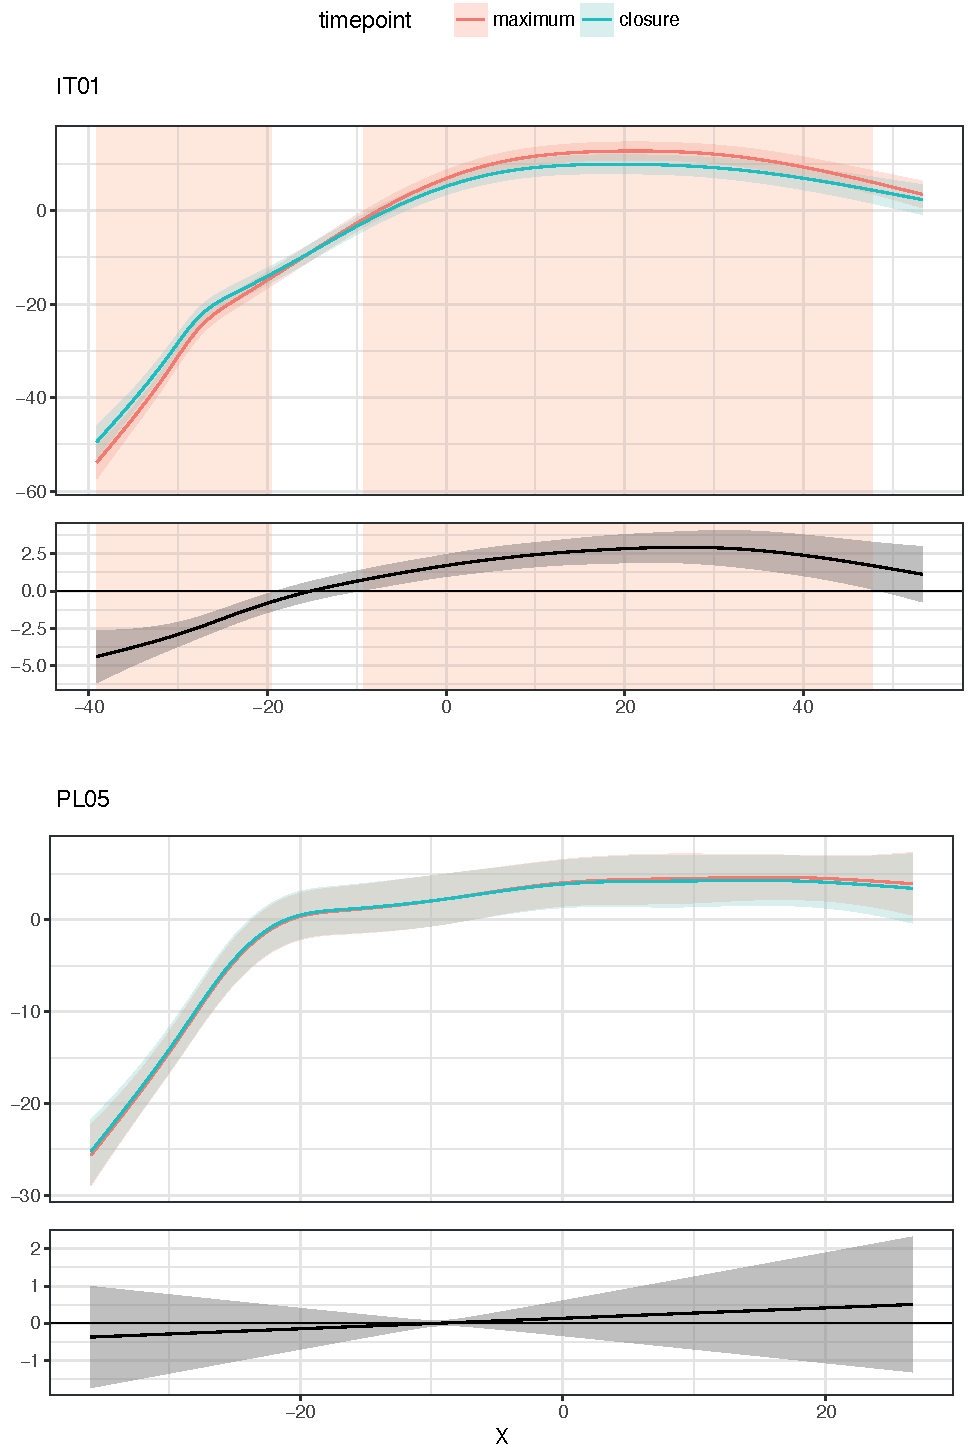
\includegraphics[width=.9\textwidth]{fig/voiced.pdf}
    \caption{Comparison of tongue contours of voiced consonants at C2 closure onset and maximum tongue displacement (within C2 closure) in IT01 (Italian) and PL05 (Polish). See \Cref{s:splines} for more details.}
    \label{f:voiced}
\end{figure*}

The ultrasonic data also showed that the tongue body was raised in
speakers with tongue root advancement. The presence of this additional
gesture makes sense from an anatomical point of view. Raising the tongue
body is a way to counterbalance the compression of the tongue mass
caused by the advancement of the root
\citep{perkell1969, jackson1988, sproat1993, kingston1997, fulop1998}.
It is not thus surprising to observe a raised tongue body in voiced
stops accompanying root advancement.

\section{Discussion}\label{discussion}

\label{s:discussion}

Based on the previously established link between tongue root advancement
and voicing, it was proposed at the beginning of this paper that the
presence of the voicing effect in a language should be correlated with
the presence of tongue root advancement in the voiced stops of that
language. To test the correlation between tongue root advancement and
vowel durations, ultrasonic data were collected from speakers of two
languages that differ in the presence/absence of the voicing effect,
Italian and Polish respectively. It was predicted that voiced consonants
should be produced with an advanced tongue root in Italian, but not in
Polish. The results of this study indicate that tongue root advancement
in voiced stops correlates with the presence of the voicing effect,
although the details of such correlation reveal a more complex picture.

\citet{keating1984} investigated the effect of consonant voicing on the
duration of preceding vowels and reported that vowels followed by
voiceless and voiced stops do not differ in duration. Nevertheless, the
analysis of the durational data discussed above indicates that an effect
of voicing exists in the Polish speakers of this study, such that vowels
followed by voiced stops are on average 8 milliseconds longer. The
hypothesis that voiced consonants should not have tongue root
advancement in Polish rests on the notion that Polish has been reported
as a non-voicing-effect language. The data from this study indicate
instead the presence of a voicing effect. Crucially, the Polish speaker
with the strongest effect of voicing (PL05, cf. \Cref{s:vow-duration})
is also the only Polish speaker who produced voiced consonants with an
advanced tongue root, both at C2 closure onset and at the time of
maximum tongue displacement.

This pattern is similar to that of the Italian speakers, who have both a
relatively strong voicing effect and tongue root advancement. This is
true for all the speakers of Italian in this sample, except IT04. The
vowels in this speaker are 22 milliseconds longer when followed by
voiced stops, but her tongue root position does not differ in voiced and
voiceless stops. In \Cref{s:source}, I briefly discuss a tentative
explanation for the different behaviour of IT04.

Overall, the speakers who produced voiced consonants with an advanced
tongue root had a relatively strong voicing effect, with estimates of
the durational differences ranging between 15 and 30 milliseconds. Bear
in mind that the inverse is not true: IT04 had a strong voicing effect,
without accompanying tongue root advancement. Nonetheless, the
generalisation that tongue root advancement is correlated with a
relatively strong voicing effect holds independently of the speaker's
language: speakers of both Italian and Polish pattern according to this
principle. All things considered, the following implication can be
inferred: if a speaker realises voiced consonants with concomitant
advancement of the tongue root, other things being equal, then that same
speaker will also show a considerable durational difference in vowels,
with longer vowels preceding voiced consonants.

The fact that the degree of tongue advancement at C2 closure onset and
at maximum displacement does not differ in PL05's voiced consonants
could be linked to the relative weaker effect of voicing in this speaker
compared to the Italian speakers (14 vs 22 milliseconds). The weaker
voicing effect in PL05 suggests that the relationship between tongue
root advancement and vowel duration might be gradient rather then
categorical (presence vs.~absence). If this is the case, the magnitude
of the voicing effect should correlate with the degree of tongue root
advancement. More specifically, vowel duration is predicted to be
directly correlated with the degree of advancement. Future work will set
out to investigate the putative gradient effect of tongue root
advancement on vowel duration.

Having demonstrated that tongue root advancement in voiced stops is
associated with a relatively stronger voicing effect, we can now move to
discuss tongue root advancement as the precursor of the voicing effect.
As pointed out in \Cref{s:intro}, the source of the voicing effect
should be found among the supra-glottal articulatory properties of
stops. Such putative source should also be subject to language- and/or
speaker-specific behaviour. As evinced by the data presented here,
tongue root advancement satisfies both of these requirements.

Tongue root advancement as an oral gesture does not need discussion,
since it involves a lingual articulation. As for the second requisite,
the results of this study show that speakers can adopt tongue root
advancement or not, but, if they do, they do so in such a way that the
root in voiced stops is already advanced at the onset of the consonant
closure. The most straightforward interpretation is that the advancement
of the root is initiated before the consonant closure is achieved. This
implies that the advancement gesture is implemented even during the
articulation of the vowel. Adapting the reasoning of the proposal by
Halle and Stevens (1967, see \Cref{s:intro}), a possible source of the
longer duration of vowels before voiced consonants could therefore be
the additional time required to achieve tongue root advancement in the
context of voiced stops.

Such gestural account is intended as a diachronic source of the voicing
effect, rather than as a mechanic condition according to which the
voicing effect should be observed synchronically. This is in compliance
with the fact that one speaker of Italian did not produce voiced
consonants with tongue root advancement, while still having a relatively
strong voicing effect. A speculative explanation is that, once a strong
voicing effect is stabilised in a language (or a variety of a language),
speakers of that language will learn the effect while being able to
adopt different strategies to cope with the decreasing trans-glottal
pressure drop.

To conclude, the gestural-timing account proposed here confers a more
salient function to the size of the effect of voicing on vowel duration.
If present, tongue root advancement is expected to co-occur with a
relatively stronger voicing effect. As we saw earlier, the presence of
tongue root advancement in the Polish speaker PL05 was accompanied by an
8 millisecond increase in the degree to which voicing affects vowel
duration. This aspect, coupled with the hypothesis explored above that
the effect of voicing on vowel duration could be gradient, evidently
illustrates the complexity of this phenomenon, that has being escaping
our understanding for almost a century.

\section{Conclusion}\label{conclusion}

\label{s:conclusion}

This paper focussed on the so called voicing effect, by which vowels
tend to be longer before voiced than before voiceless stops in a variety
of languages. No consensus has been reached in the literature regarding
the source of this effect. On the other hand, voicing in stops has long
been known to be facilitated by pharyngeal cavity expansion, which is
often implemented by means of tongue root advancement. I therefore
offered the hypothesis that tongue root advancement in voiced stops
might play a role in determining the presence vs.~absence of the voicing
effect in a particular language.

Drawing on acoustic and ultrasonic data from Italian (a voicing-effect
language) and Polish (a non-voicing-effect language), I showed that:

\begin{itemize}
\tightlist
\item
  Vowels in Polish are on average 6 milliseconds longer when followed by
  voiced stops.
\item
  In Italian, vowels are on average 22 milliseconds longer before voiced
  stops.
\item
  Voiced stops were realised with tongue root advancement in three
  Italian speakers and one Polish speaker.
\item
  The durational increment in the Polish speaker with tongue root
  advancement is double compared to the other Polish speakers, although
  still smaller than that of the Italian speakers.
\item
  Tongue root advancement was found both during the closure and at the
  time of closure onset of voiced consonants, both in the Italian and
  the Polish speakers showing root advancement.
\item
  The degree of root advancement increases during closure in the Italian
  speakers but not in the Polish speaker.
\end{itemize}

These results indicate that tongue root advancement is correlated with
vowel duration, although in a unexpected way. More specifically, I found
that, independent of language, the difference in vowel duration was
greater in speakers who produce voiced consonants with tongue root
advancement, than in speakers without tongue root advancement. Following
from this, I advanced the hypothesis that the relation between the
degree of tongue root advancement and the magnitude of the voicing
effect is gradient rather than a matter of presence vs.~absence.
Finally, I speculated that the additional time required for the tongue
root to reach an advanced position is a possible diachronic precursor of
the longer duration of vowels preceding voiced stops.

\bibliography{linguistics.bib}

\end{document}
